\documentclass[problem]{mcs}

\begin{pcomments}
  \pcomment{PS_3color_SAT}
  \pcomment{by ARM October 25, 2011, edited with new figure 4/4/12}
\end{pcomments}

\pkeywords{
SAT
logical_formula
propositional_logic
logic
proposition
negation
coloring
}

%%%%%%%%%%%%%%%%%%%%%%%%%%%%%%%%%%%%%%%%%%%%%%%%%%%%%%%%%%%%%%%%%%%%%
% Problem starts here
%%%%%%%%%%%%%%%%%%%%%%%%%%%%%%%%%%%%%%%%%%%%%%%%%%%%%%%%%%%%%%%%%%%%%

\begin{problem}
This problem will show that 3-coloring a graph is just as difficult as
finding a satisfying truth assignment for a propositional formula.
The graphs considered will all be taken to have three designated
\emph{color-vertices} connected in a triangle to force them to have
different colors in any coloring of the graph.  The colors assigned to
the color-vertices will be called $T,F$ and $N$.

Suppose $f$ is an $n$-argument truth function.  That is,
\[
f:\set{T,F}^n\to \set{T,F}.
\]
A graph $G$ is called a \emph{3-color-\textit{f}-gate} iff $G$ has $n$
designated \emph{input vertices} and a designated \emph{output
  vertex}, such that

\begin{itemize}

\item $G$ can be 3-colored \emph{only} if its input vertices are
  colored with $T$'s and $F$'s.

\item For every sequence $b_1,b_2,\dots, b_n \in \set{T,F}$, there is
  a 3-coloring of $G$ in which the input vertices $v_1,v_2,\dots,
  v_n\in \vertices{G}$ have the colors $b_1,b_2,\dots, b_n \in
  \set{T,F}$.

\item In any 3-coloring of $G$ where the input vertices
  $v_1,v_2,\dots, v_n\in \vertices{G}$ have colors $b_1,b_2,\dots, b_n
  \in \set{T,F}$, the output vertex has color $f(b_1,b_2,\dots, b_n)$.

\end{itemize}

For example, a 3-color-$\QNOT$-gate consists simply of two adjacent
vertices.  One vertex is designated to be the input vertex, $P$, and
the other is designated to be the output vertex.  Both vertices have
to be constrained so they can only be colored with $T$'s or $F$'s in
any proper 3-coloring.  This constraint can be imposed by making them
adjacent to the color-vertex $N$, as shown in
Figure~\ref{fig:3color-NOT}.

\begin{figure}\inbook{[h]}
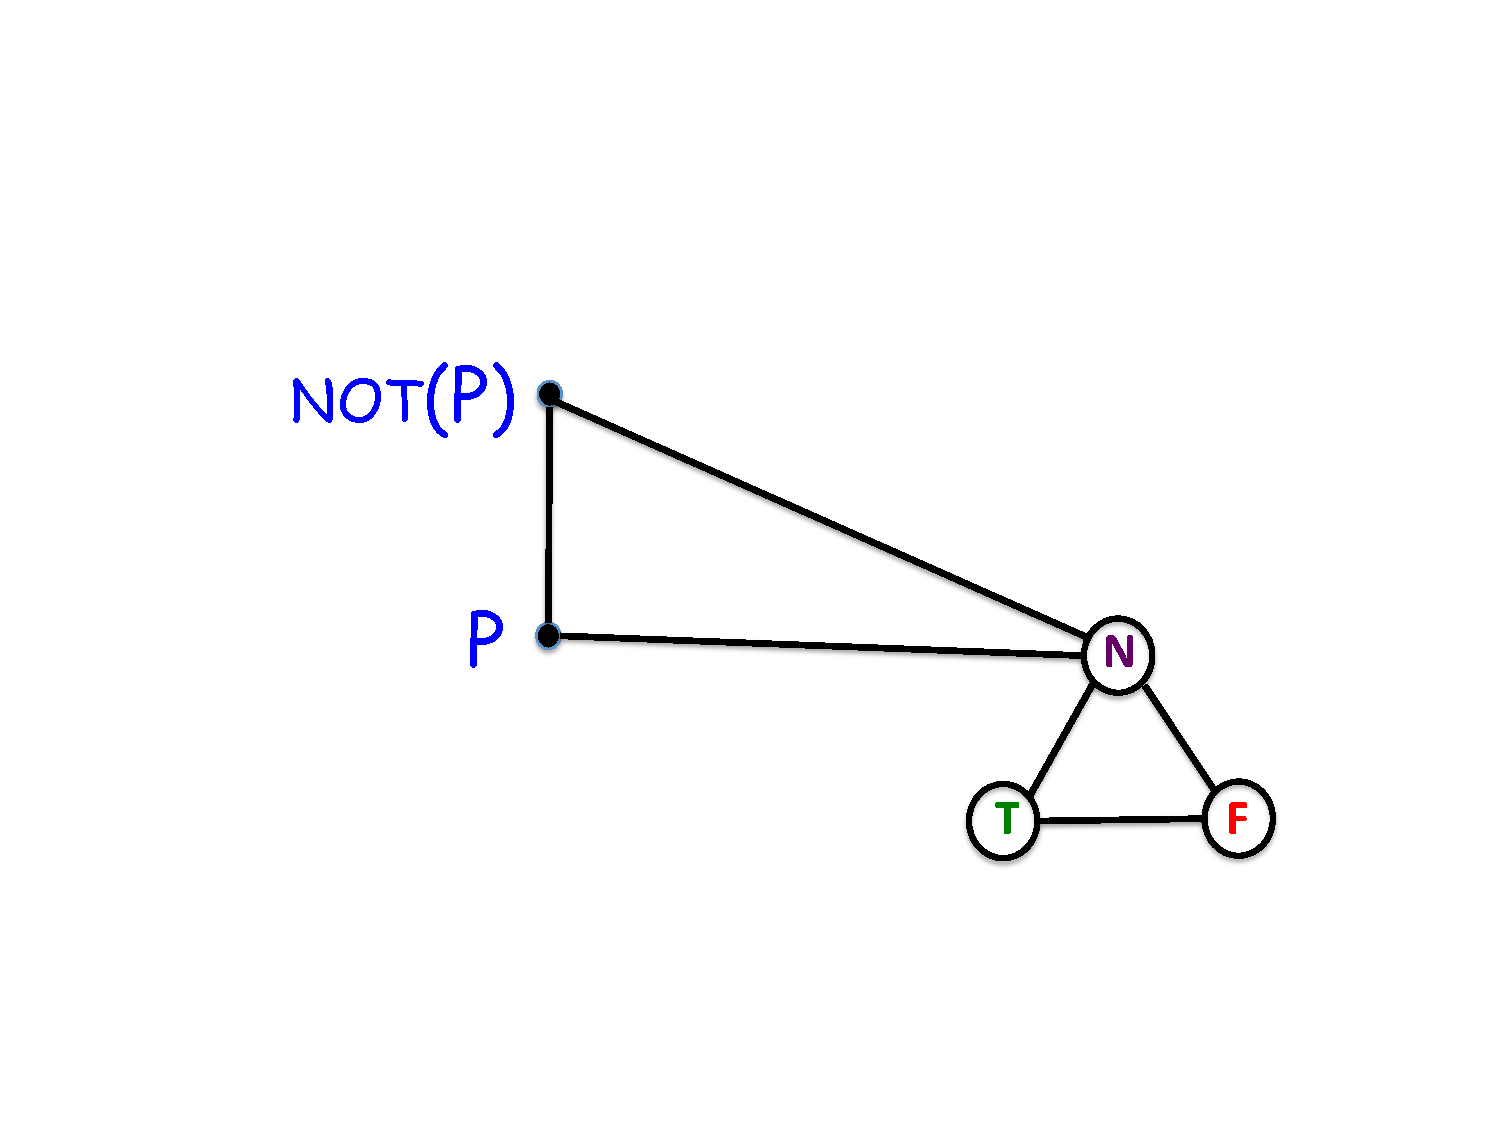
\includegraphics[width=4in]{3color-NOT}
\caption{A 3-color $\QNOT$-gate}
\label{fig:3color-NOT}
\end{figure}

\begin{figure}\inbook{[h]}
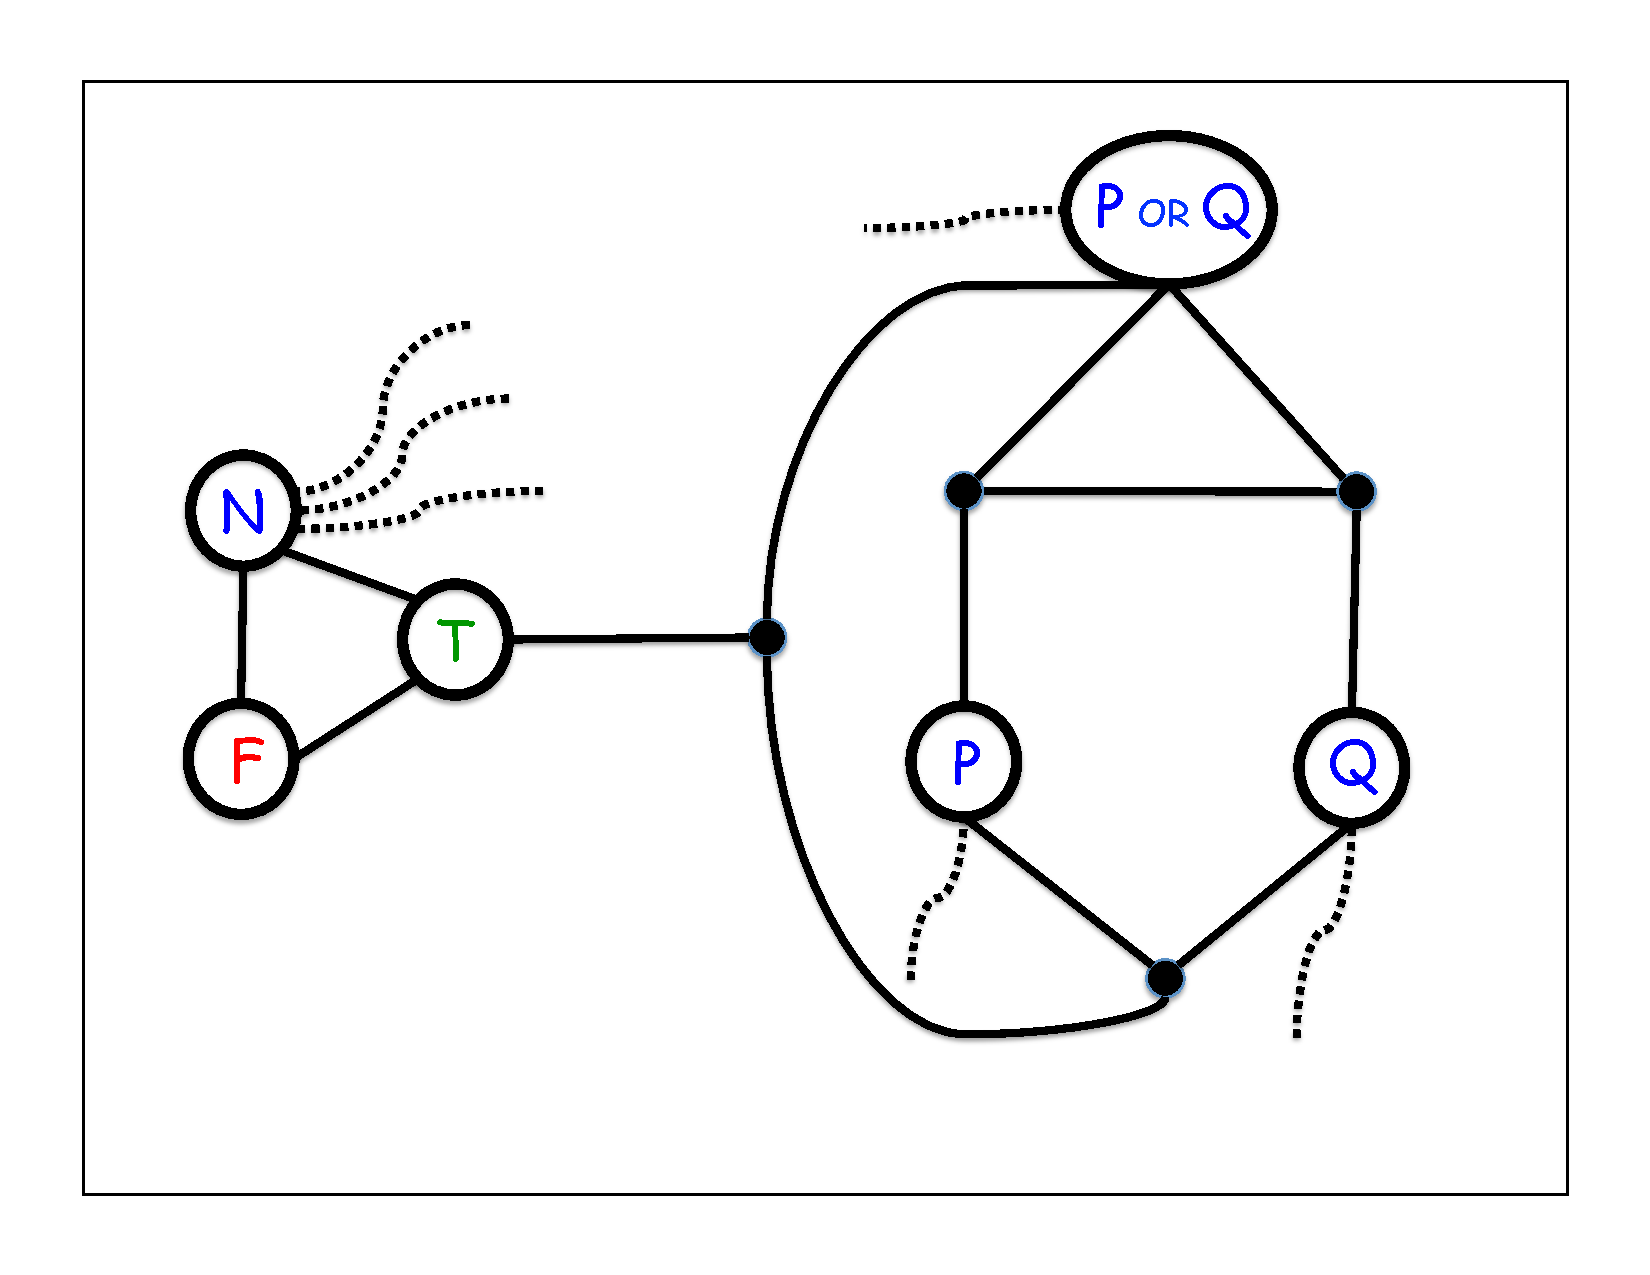
\includegraphics[width=4in]{3color-OR}
\caption{A 3-color $\QOR$-gate}
\label{fig:3color-OR}
\end{figure}

\inhandout{\newpage}

\bparts

\ppart Verify that the graph in Figure~\ref{fig:3color-OR} is a
3-color-$\QOR$-gate.  (The dotted lines indicate edges to color-vertex
$N$; these edges constrain the $P$, $Q$ and $P \QOR Q$ vertices to be
colored $T$ or $F$ in any proper 3-coloring.)

\begin{solution}
The diagram is symmetric in $P$ and $Q$, so there only three cases to
consider: $P$ and $Q$ are both colored $T$, both colored $F$, or $P$
and $Q$ are colored differently.  If $P$ and $Q$ are colored
differently, there is only one possible 3-coloring and the output
vertex labelled ``$P \QOR Q$'' is colored $T$.

If $P$ and $Q$ have the same color, then one of the vertices directly
above must be colored with $N$ and the other with the $\QNOT$ of the
color of $P$ and $Q$.  This forces the $P \QOR Q$ vertex to be colored
with the same color as $P$ and $Q$.  There is then a unique coloring
of the bottom vertex and the middle vertex on the arc on the left that
can complete a three coloring.
\end{solution}

\ppart\label{fgateforNOTOR} Let $E$ be an $n$-variable propositional
formula, and suppose $E$ defines a truth function $f:\set{T,F}^n\to
\set{T,F}$.  Explain a simple way to construct a graph that is a
3-color-\textit{f}-gate.

\begin{solution}
A recursive construction is straightforward, using the fact that every
propositional connective can be expressed in terms of $\QOR$ and
$\QNOT$.  For example, suppose $E$ is of the form $G \QOR H$ for
propositional formulas $G$, $H$.  So if $G$ and $H$ define truth
functions $g$, $h$, then $f = g \QOR h$.

To construct a 3-color-\textit{f}-gate, recursively construct a
3-color-\textit{g}-gate and a 3-color-\textit{h}-gate, each built
starting from the same $n$ vertices corresponding to the $n$ variables
in $E$.  Then construct a new 3-color-$\QOR$-gate as in
Figure~\ref{fig:3color-OR} using new vertices except that the output
vertex of the 3-color-\textit{g}-gate will be the $P$ vertex in the
new 3-color-$\QOR$-gate, the output vertex of the
3-color-\textit{h}-gate will be the $Q$ vertex in the new
3-color-$\QOR$-gate.  Then designate the $P \QOR Q$ vertex of in the
new 3-color-$\QOR$-gate to be the output vertex of the
3-color-\textit{f}-gate.
\end{solution}

\ppart Explain why an efficient procedure for determining if a graph
was 3-colorable would lead to an efficient procedure to solve the
satisfiability problem, SAT.

\iffalse
\hint To determine if propositional formula, $E$, is satisfiable, use
the construction from Problem~\bref{PS_equisatisfiable_3CNF} to find a
formula $J$ using only $\QNOT$ and $\QOR$ such that $J$ is satisfiable
iff $E$ is satisfiable.
\fi

\begin{solution}
To determine if an $n$-variable propositional formula, $E$, that
defines a truth function $f:\set{T,F}^n\to \set{T,F}$, is satisfiable,
use the construction in part~\eqref{fgateforNOTOR} to construct a
3-color-\textit{f}-gate.

Then add an edge between the output vertex of the
3-color-\textit{f}-gate and the $F$-colored vertex.  This
constrains the output vertex to be $T$ is any 3-coloring of the
3-color-\textit{f}-gate.  Call this graph $G$.  So $G$ is 3-colorable
iff there is a coloring of the input vertices that makes the output
vertex color $T$, and this is possible iff $E$ is satisfiable.
Moreover, the whole construction of $G$ can essentially be done in
time proportional to the size of $E$, so an efficient procedure to
test $G$ for 3-colorability would yield an efficient procedure to test
$E$ for satisfiability.

\iffalse

Problem~\bref{PS_equisatisfiable_3CNF} to find a 3-CNF
formula, $H$, that is satisfiable iff $E$ is satisfiable.  Then
construct a formula $J$ equivalent to $H$ using DeMorgan's law to
replace the $\QAND$'s in $H$.  Since each application of DeMorgan's
Law replaces a $\QAND$ by two $\QNOT$'s and a $\QOR$, the formula $J$
is easy to construct from $H$ and uses at most three times as many
operations as $H$.  Now build a 3-color-\textit{f}-gate for $J$ using
part~\eqref{fgateforNOTOR}.  Finally, add an edge between the output
vertex of the 3-color-\textit{f}-gate and the $F$-colored vertex; call
this graph $K$.  So $K$ is 3-colorable iff there is a coloring of the
input vertices that makes the output vertex color $T$ which is
possible iff $J$ and hence $H$ and $E$ are satisfiable.  Moreover, the
whole construction of $K$ from $E$ can essentially be done in time
proportional to the size of $E$, so an efficient procedure to test
$K$ for 3-colorability would yield an efficient procedure to test $E$
for satisfiability.
\fi


\end{solution}

\eparts

\end{problem}

%%%%%%%%%%%%%%%%%%%%%%%%%%%%%%%%%%%%%%%%%%%%%%%%%%%%%%%%%%%%%%%%%%%%%
% Problem ends here
%%%%%%%%%%%%%%%%%%%%%%%%%%%%%%%%%%%%%%%%%%%%%%%%%%%%%%%%%%%%%%%%%%%%%

\endinput
